\documentclass[10pt]{article}
\usepackage[margin=0.9in]{geometry}
\usepackage{amsmath,booktabs,graphicx,hyperref}
\title{Noise-Resolved Physical Contrasts for Dexterous Interaction Models:\\A Pilot Study of Measurement and Actor-Panel Transfer}
\author{Working manuscript}
\date{1 October 2026}
\begin{document}
\maketitle
\noindent\textbf{Status.} Exploratory working draft. The experiments below do not establish a new
state-of-the-art method, causal policy improvement, or a journal-ready claim.

\begin{abstract}
Interaction models intended for dexterous control must distinguish the consequences of
candidate actions, rather than merely predict observed motion. Before learning these
differences, their physical measurement must also be resolved against repeated-process
variation. We implement a cold-start replay diagnostic with one-step wrist translation
interventions in an existing self-trained Inspire-hand simulation substrate. Four panels,
each containing 96 environments across three airplane reference motions, are evaluated
under two zero interventions and positive and negative 10-mm requested PD-target offsets.
At five and ten control steps, the pooled position-response contrasts are 7.15 and
18.83 mm RMS, compared with 0.10 and 0.44 mm for zero-intervention repeats. However,
vertical response is not consistently positive across panels, failing the predeclared
joint physical screen. A separately documented vector-prediction screen then fits matched
factual, differential-loss and no-pulse-input networks on one frozen actor's panels and
evaluates on another's. Across three optimization seeds, differential-loss contrast errors
are 10.11 and 26.99 mm, with no improvement over strong simple controls. These pilots
separate measurable action effects from beneficial lift and from transferable learned
effects. They motivate further work on contact-specific data coverage, while providing
no evidence of manipulation-policy utility.
\end{abstract}

\section{Introduction}
Human hand--object data and simulated robotic rollouts offer substantial supervision for
interaction dynamics. A predictive representation can nevertheless fail to improve a
control decision. Prediction may capture common reference motion, while useful action
selection depends on much smaller differences between feasible interventions. A second
issue is experimental resolution: two closed-loop evaluations can have nearly identical
aggregate success rates but disagree about which episodes succeed. Measurement quality,
learning quality and task benefit therefore require separate checks.

The existing repository contains self-trained manipulation actors, object-centric motion
models, cross-source geometry and intervention tooling. Its prior four-seed effect-rank
validation does not support the joint positive action-alignment and policy-utility claim.
A subsequent frozen-actor audit reports 34 versus 35 successes among 384 paired episodes,
but 63 discordant success labels. These are inherited records, not newly validated
results of this paper. They motivate measuring shorter physical responses before
committing further resources to a controller.

Particle representations already support cross-embodiment world modeling and planning
\cite{he2025}. Value-aware model learning \cite{farahmand2017} and action-discriminative
world models \cite{qiu2026} explicitly connect predictions to decisions. Controllability
representations also have established foundations \cite{rudolph2024}. We do not claim
novelty for those general ideas. This pilot asks a narrower question: when a small action
intervention is physically resolvable in a contact-rich substrate, does a simple
contrast-supervised predictor transfer its effect to another actor's replay panels?

\section{Physical-response measurement}
For a recorded action sequence, let $\tau_i$ be the control step immediately after the
first reference event where both the native hand-force and object-force proxies are active.
This retrospective diagnostic schedule does not establish pairwise hand--object contact.
For environment $i$, amplitude $u\in\{-0.01,0,0.01\}$ modifies only wrist-$z$ normalized
action at $\tau_i$. The native translation scale is one, giving a requested target
offset of $u$ meters. Actual wrist motion is governed by the PD controller and contact
physics; it is not asserted to equal the requested offset. All later actions follow
the identical recorded sequence.

Define the response relative to each run's actual pre-intervention state as
\begin{equation}
 R_{i,H}^{u}=p_{i,\tau_i+H}^{u}-p_{i,\tau_i}^{u},
 \qquad D_{i,H}=R_{i,H}^{+}-R_{i,H}^{-}.
\end{equation}
Two zero-intervention processes give the repeat contrast
$N_{i,H}=R_{i,H}^{0a}-R_{i,H}^{0b}$. We report
\begin{equation}
 S_H=\sqrt{n^{-1}\sum_i\|D_{i,H}\|_2^2},\quad
 B_H=\sqrt{n^{-1}\sum_i\|N_{i,H}\|_2^2}.
\end{equation}
The descriptive ratio $S_H/B_H$ is reported only when $B_H>0$. A zero observed repeat
difference does not establish zero process uncertainty or infinite measurement quality.
It is encoded as an undefined ratio.

The DExplore simulation substrate \cite{xu2025} uses self-trained actors in this study.
Each process starts from the same archived cold simulator state, with physical-property,
root/DOF, observation, recurrent-state and RNG checks inherited from the paired evaluator.
No warm PhysX solver state is claimed to be restorable. Recorded per-step RNG schedules
and normalized actions are replayed. Four panels combine actor training seeds 286/287
with evaluation seeds 288/289; each panel has 32 environments per motion. These
384 windows are not 384 independent motions or training seeds. The predeclared physical
screen requires $S_H/B_H\ge2$ at $H=5,10$, and positive mean vertical contrast in every
panel at both horizons. This is an operational Probe gate, not a statistical confidence
guarantee. The matrix has no failures or excluded runs.

\section{Vector-prediction screen}
After the physical screen fails its directional component, a documented decision retains
that failure and permits a separate test of full vector-response prediction. Its reused
test panels were already included in physical diagnostics; they are not a pristine
Validation set. Optimization and normalization nevertheless exclude all actor-287 rows.

The fit/test sets contain 192 windows each, from actor 286/287 respectively. A window has
four intervention arms. Inputs comprise four actual past/current 55-dimensional physical
states and masks, followed by ten predetermined normalized 18-dimensional action vectors
beginning at the intervention. Future observed physical states never enter the features.
The action sequences are retrospective replay banks, not deployable future actor actions.
Targets are three-dimensional position responses at five and ten steps.

All learned models use two 128-unit SiLU hidden layers and six outputs. Three initialization
seeds (301--303) each train factual, differential and no-pulse models for exactly 1000 Adam
updates, learning rate $10^{-3}$, with matched 96-window mini-batches. No checkpoint is
selected using test errors. Normalization and loss scales use fit data only. Factual
training minimizes normalized response MSE. Differential training adds coefficient-one
MSE on predicted plus--minus contrasts, scaled by fit contrast RMS. The no-pulse model
substitutes the zero-arm plan, retaining actual observed history and the common replay
plan but hiding the assigned pulse. Additional controls predict the global fit mean
contrast and a privileged per-motion fit mean contrast.

The fixed learning gate requires, at both horizons, at least 10\% lower seed-mean contrast
RMSE than the factual model and global fit-mean control, and at least 75\% agreement with
the measured vertical contrast's sign. Sign agreement concerns the observed sign, not
an assumption that every effect should be positive. Optimization seeds quantify variation
of this small fitting procedure; they are not independent policy-training replications.

\section{Results}
\begin{table}[h]
\centering
\caption{Physical contrast measurements, pooled over the four fixed panels. Requested
PD target offsets differ by 20 mm between positive and negative arms.}
\begin{tabular}{rrrrr}
\toprule
Steps & Seconds & Pulse RMS (mm) & Repeat RMS (mm) & Ratio\\
\midrule
1 & 0.033 & 1.914 & 0.000 & undefined\\
2 & 0.067 & 2.572 & 0.084 & 30.75\\
5 & 0.167 & 7.150 & 0.101 & 70.44\\
10 & 0.333 & 18.827 & 0.444 & 42.36\\
20 & 0.667 & 75.463 & 6.081 & 12.41\\
30 & 1.000 & 105.792 & 9.638 & 10.98\\
\bottomrule
\end{tabular}
\end{table}

Physical-resolution subgates pass, but vertical contrasts have mixed signs. At five steps,
panel means are $-0.025$, $0.009$, $-0.108$ and $0.845$ mm; at ten steps they are
$-0.028$, $0.005$, $-0.303$ and $0.253$ mm. The joint physical screen is therefore
\texttt{UNPROMISING}. Large three-dimensional response is not evidence that lifting the
wrist improves object lift. Pre-intervention plus--minus position mismatch is zero
in three panels and 0.012 mm RMS in the remaining panel. This measures exposed state
agreement and does not establish equality of hidden solver state.

\begin{figure}[h]
\centering
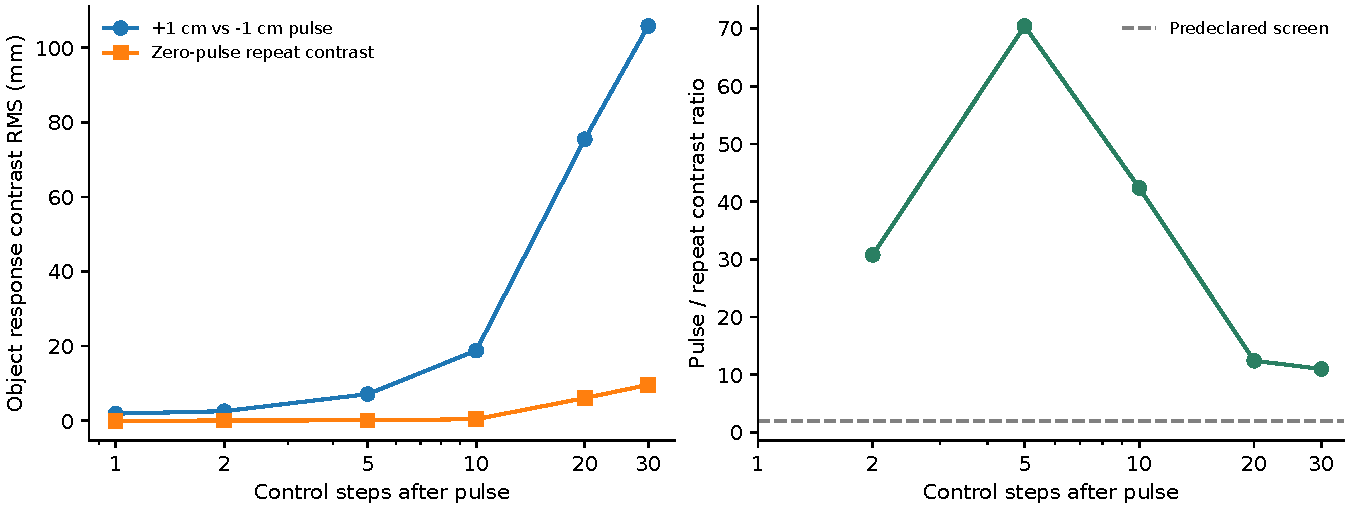
\includegraphics[width=\linewidth]{figures/contact_response.pdf}
\caption{Physical pulse and repeat contrasts. Ratios summarize the observed repeat pair
only; they are not calibrated signal-to-noise estimates or confidence bounds.}
\end{figure}

\begin{table}[h]
\centering
\caption{Actor-287 contrast RMSE in millimeters. Learned rows average the three fixed
optimization seeds. The motion control uses privileged motion identity.}
\begin{tabular}{lrr}
\toprule
Model & Five steps & Ten steps\\
\midrule
Factual & 10.121 & 26.546\\
Differential & 10.114 & 26.990\\
No-pulse input & 9.922 & 26.456\\
Global fit mean & 10.061 & 26.259\\
Per-motion fit mean & 10.137 & 26.340\\
\bottomrule
\end{tabular}
\end{table}

Differential training changes mean error by less than 0.1\% relative to factual training
at five steps and increases it by approximately 1.7\% at ten steps. It does not beat
the global-mean baseline. Its measured vertical-sign agreement is 32.6\% and 31.1\%,
below the fixed 75\% gate. Every component of the learning screen fails, so this
implementation is also \texttt{UNPROMISING}. The complete physical matrix took
481.9 seconds, and the nine GPU fits plus preprocessing and evaluation took 17.2 seconds.
One RTX 3090 was used. Combined run artifacts occupied approximately 70 MB before
the manuscript export.

\section{Discussion and limitations}
The physical and learning screens answer different questions. The pulse experiment
shows differences larger than observed zero-replay contrasts in this fixed substrate.
It does not show that a representation can infer those differences in new settings.
The learned screen directly fails to establish such transfer for the tested small model.
Neither observation identifies the cause of failure. Sparse contact-state coverage,
distribution change between actors, feature insufficiency and optimization remain
candidate explanations; this study does not select among them.

Contact proxies can activate because the hand and object independently contact the
table. A future measurement protocol should validate actual interacting geometry or
pairwise contact information. Shared cold conditions and replay actions also do not
clone hidden contact solver state. Run order is fixed, with only one positive and one
negative process per panel, limiting treatment/noise separation. No population-level
confidence interval is claimed, and no inferential advantage is inferred from the
nominal count of 384 repeated windows.

The studied object and reference motions are shared between fitting and evaluation.
The action banks are diagnostic and involve only one wrist direction. There is no
learned rollout controller, matched Cm-on/off policy training, real-world experiment,
unseen-object test, or cross-hand test in these pilots. Strong geometric and model-based
control baselines would be required before attributing benefit to a new interaction
representation. The results cannot justify a journal-level generalization or utility
claim. Any proposed future method must also be distinguished from established
cross-embodiment, value-aware and action-bisimulation approaches.

\section{Conclusion and next research decision}
The tested short-horizon physical effects are measurable, but a monotone wrist-lift
interpretation fails and the tested differential predictor does not transfer across
the frozen actor panels. We retain both negative Probe decisions and stop this
small-data model rather than increasing its updates or selecting another seed.
The next consequential question is whether verified contact-conditioned coverage
changes predictability on newly collected, independently frozen test data. Policy
and hardware utility would remain separate required validations even after a positive
predictive result.

\section*{Reproducibility}
The study is isolated in \texttt{agent/contact-response-cm}. Physical execution is
fixed to commit \texttt{466e80d}; learning execution to \texttt{44f22ea}.
Run manifests record input/output hashes, commands, GPU UUID, process status and budgets.
Original checkpoints, motion data and previous audits are read-only inputs.
Raw compact physical traces, nine fitted networks and test predictions are retained.
The authoring script exports tables directly from the recorded JSON results. The
source repository's original working tree remains on \texttt{agent/paired-evaluator}.

\begin{thebibliography}{9}
\bibitem{he2025} Z. He et al. Scaling Cross-Embodiment World Models for Dexterous Manipulation.
arXiv:2511.01177, 2025. \url{https://arxiv.org/abs/2511.01177}.
\bibitem{xu2025} S. Xu et al. Dexplore: Scalable Neural Control for Dexterous Manipulation
from Reference-Scoped Exploration. CoRL, 2025. \url{https://arxiv.org/abs/2509.09671}.
\bibitem{farahmand2017} A.-M. Farahmand, A. Barreto and D. Nikovski. Value-Aware Loss Function
for Model-based Reinforcement Learning. AISTATS, 2017.
\url{https://proceedings.mlr.press/v54/farahmand17a.html}.
\bibitem{qiu2026} J. Qiu et al. AD-WM: Action-Discriminative World Models for Counterfactual
Model Predictive Control. arXiv:2609.30264, 2026. \url{https://arxiv.org/abs/2609.30264v2}.
\bibitem{rudolph2024} M. Rudolph et al. Learning Action-based Representations Using Invariance.
Reinforcement Learning Journal, 2024.
\url{https://rlj.cs.umass.edu/2024/papers/RLJ_RLC_2024_39.pdf}.
\end{thebibliography}
\end{document}
